\documentclass[10pt,twocolumn]{article}
\usepackage{times}
\usepackage{multirow}
\usepackage{tabularx}
\usepackage{subcaption}
\usepackage{graphicx,grffile}
\usepackage{pgf}
\usepackage{tikz}
\usetikzlibrary{arrows,automata}
\usepackage[latin1]{inputenc}

% do not change these values
\baselineskip 12pt
\textheight 9in
\textwidth 6.5in
\oddsidemargin 0in
\topmargin 0in
\headheight 0in
\headsep 0in

%\makeatletter
%\def\maxwidth{\ifdim\Gin@nat@width>\linewidth\linewidth\else\Gin@nat@width\fi}
%\def\maxheight{\ifdim\Gin@nat@height>\textheight\textheight\else\Gin@nat@height\fi}
%\makeatother
%% Scale images if necessary, so that they will not overflow the page
%% margins by default, and it is still possible to overwrite the defaults
%% using explicit options in \includegraphics[width, height, ...]{}
%\setkeys{Gin}{width=\maxwidth,height=\maxheight,keepaspectratio}
%

\usepackage[unicode=true]{hyperref}
\hypersetup{breaklinks=true,
            bookmarks=true,
            pdfauthor={},
            pdftitle={},
            colorlinks=true,
            citecolor=blue,
            urlcolor=blue,
            linkcolor=blue,
            pdfborder={0 0 0}}
\urlstyle{same}  % don't use monospace font for urls

\usepackage[font=footnotesize,labelfont=bf]{caption}

\begin{document}

\title{outline!}

\author{
%Noah Watkins, Neha Ojha\textsuperscript{*}, Carlos Maltzahn \\
%\small {\em University of California, Santa Cruz} \\
%\small {\{jayhawk,carlosm\}@cs.ucsc.edu} \textsuperscript{*}nojha@ucsc.edu \\ [2mm]
\small Submission Type: Research
}

\date{}
\maketitle

\begin{abstract}
To meet the needs of a diverse and growing set of cloud-based applications,
modern distributed storage frameworks expose a variety of composable
subsystems as building blocks.  This approach gives infrastructure programmers
significant flexibility in implementing application-specific semantics while
reusing trusted components.  Unfortunately, in current storage systems the
composition of subsystems is a low-level task that couples (and hence
obscures) a variety of orthogonal concerns, including functional correctness
and performance.  Building an application by wiring together a collection of
components typically requires thousands of lines of carefully-written C++
code, an effort that must be repeated whenever device or subsystem
characteristics change.

In this paper, we propose a declarative approach to subservice composition
that allows programmers to focus on the high-level functional properties that
are required by applications.  Choosing an implementation that is consistent
with the declarative functional specification then can be posed as a search
problem over the space of parameters such as block sizes, storage interfaces
(e.g. key/value or block storage) and concurrency control mechanisms.  We
present experimental evaluation of our prototype, (etc etc)
\end{abstract}

\section{Introduction}

% whats the problem
Storage systems are increasingly providing features that take advantage of
application-specific knowledge to achieve optimizations and provide unique
services. However, this trend is leading to the creation of a large number of
software extensions that will be difficult to maintain as system software and
hardware continue to evolve.

% why is it interesting
The standardization of the POSIX file I/O interface has been a major success,
allowing application developers to avoid vendor lock-in. However, large-scale
storage systems have been dominated by proprietary products, preventing
exploration of alternative interfaces and complicating future migration paths,
eliminating the benefits of commodity systems. But the recent availability of
high-performance open-source storage systems is changing this because these
systems are modifiable, enabling interface change, and reducing the risks of
lock-in. The widely deployed Ceph distributed storage system is an example of
a storage system that supports application-specific extensions in the form of
custom I/O interfaces to objects managed by the underlying RADOS object
storage system~\cite{weil:osdi06,weil:pdsw07}. Organizations are increasingly
reliant upon these extensions as is shown in Figure~\ref{fig:objclass-dev} by
a marked increase in the number of object operations that are packaged as part
of the Ceph distribution and widely used by internal Ceph subsystems and by
applications such as OpenStack Swift and Cinder~\cite{openstack}.

\begin{figure}[t]
  \centering
    \includegraphics[width=0.48\textwidth]{experiments/objclass-dev/output.png}
    \caption{
[\href{https://github.com/noahdesu/zlog-popper/tree/master/experiments/objclass-dev/visualize.ipynb}{source}]
Growth of officially supported, custom object interfaces in RADOS over 6
years. An \emph{operation} is a function executed in the context of an object,
and operations are grouped into different \emph{categories}
corresponding to applications or utilities, such as reference counting}
\label{fig:objclass-dev}
\end{figure}

%%% why is it hard / why do naive approaches fail
In addition to the growth in the quantity of operations in use throughout Ceph
installations, Figure~\ref{fig:objclass-dev} also depicts the amount of
low-level C++ written to implement these operations. Unfortunately, this code
is written assuming a performance profile defined by the combination of the
hardware and software versions available at the time of development.  While
the bulk of these interfaces are created by core Ceph developers with a
complete view of the performance model, this may be changing as the
development community has been receptive to outside contributions with the
recent inclusion by CERN developers of an extension for performing limited
numeric operations on object data~\cite{cls_numops}. And while Ceph has not
yet reached the point of directly exposing these features to
non-administrative users, the recent inclusion of a mechanism for dynamically
defining extensions using Lua~\cite{cls_lua} suggests that aspects of this
feature may soon appear. What is needed is support for creating storage
interfaces using a method that allows transparent optimization as the system,
application, and supporting environment evolve.

% why hasn't it been solved before / why have previous approaches failed
Previous work related to storage interface design has largely been in the
context of standardization efforts and active storage. While the later has
been specifically concerned with the creation of application-specific
interfaces and demonstrating short-term benefits, the standardization seeks to
develop a last set of interfaces. In neither case have we seen efforts focused
on extensible interfaces with portability and longevity a primary concern.

%This trend is also not limited to Ceph. AWS Lambda, Redis Lua, Redis Modules,
%KV-Drives, and Rhea, are all recent examples of storage systems embracing the
%power of including application-specific semantics.

We propose the introduction of a declarative language for building object
based interfaces that allows a storage system to meet the needs of an
application throughout the development process without requiring rewrites.

\section{Background}

In this section we highlight the salient components of Ceph, especially its
\emph{object class} feature that offers users the ability to load and execute
application-specific codes. We provide a description of our motivating
example, a high-performance distributed shared-log built upon Ceph that makes
extensive use of the object class facility, and then we present the challenges
that application developers face when using this extensibility feature offered
by the storage system.

\subsection{Ceph and Storage Programmability}
\label{sec:objclass}

Figure~\ref{fig:ceph} illustrates the collection of components commonly
referred to as Ceph. At the bottom, a cluster of 10s--10,000s \emph{object
storage devices} compose the distributed object storage system called RADOS.
Widely deployed applications such as the S3/Swift--compliant RADOS Gateway
(RGW), RADOS Block Device (RBD), and the POSIX Ceph File System are built upon
the \emph{librados} client layer that presents a fault-tolerant always-on view
of the RADOS cluster.

\begin{figure}[t]
  \centering
  \begin{subfigure}[b]{.48\linewidth}
      \centering
      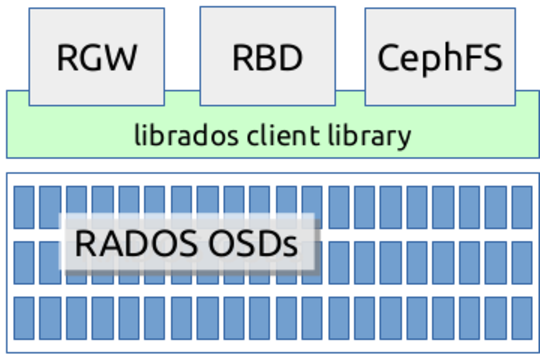
\includegraphics[width=1.0\linewidth]{figures/ceph}
      \caption{Ceph}
      \label{fig:ceph}
  \end{subfigure}\quad
  \begin{subfigure}[b]{.40\linewidth}
      \centering
      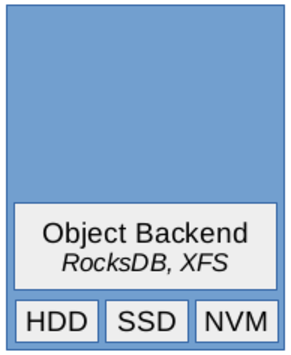
\includegraphics[width=1.0\linewidth]{figures/osd}
      \caption{OSD}
      \label{fig:osd}
  \end{subfigure}
  \caption{Ceph and OSD... gotta cram more stuff in here...}
\end{figure}

The object storage device (OSD), illustrated in Figure~\ref{fig:osd}, is the
building block of the RADOS cluster and is responsible for managing and
providing access to a set of
named objects. The configuration of an OSD is flexible, and commonly contains
a mix of commodity hardware such as HDD and SSD bulk storage, a multi-core
CPU, GBs of RAM, and one or two 10 Gb Ethernet links. Clients access object
data managed by an OSD by invoking native object operations exposed by the OSD
such as reading or writing bytes, as well as more complex operations like taking
snapshots or composing one or more native operations into compound procedures
that execute in a transactional context.

The native object operations in RADOS roughly fall into two categories based
on the type of data being accessed: key-value items, or bulk bytestream data.
The key-value interface operates as a dedicated database associated with each
object, and the bytestream interface supports random byte-level access similar
to a file.  At a
low-level each of these abstract I/O interfaces map to hardware storage
devices through a pluggable object backend storage service. For instance,
LevelDB or RocksDB may be used to store key-value data, while the
\emph{FileStore} implementation maps the bytestream interface onto a local
POSIX file system~\cite{leveldb,rocksdb}. Several backend implementations
exist for storing data in targets such as the Kinetic Drive or in NVMe devices,
among others.

%Independent of the hardware or backends chosen, Ceph allows all
%object operations to be combined to create compound operations such as storing
%key-value metadata associated with a binary blob, allowing applications to
%build object interfaces that work even as Ceph software and hardware evolve.

\paragraph*{Object Classes}
While Ceph provides a wide variety of native object operations, it also
includes a facility referred to as \emph{object classes} that allow developers
to create application-specific object operations in the form of C++ shared
libraries dynamically loaded into the OSD process at runtime.  Object classes
can be used to implement basic data management tasks such as indexing
metadata, or used to perform complex operations such as data transformations
or filtering. Table~\ref{tab:objclass-cats} summarizes the range of object
classes maintained in the upstream Ceph project which support internal Ceph
subsystems as well as applications and services that run on top of Ceph.

\begin{table}[ht]
\centering
\begin{tabularx}{\columnwidth}{|X|l|l|l|}
\hline
Category & Specialization & Methods \\ \hline
\multirow{2}{*}{Locking} & Shared & \multirow{2}{*}{6} \\
                         & Exclusive & \\ \hline
\multirow{3}{*}{Logging} & Replica & 3 \\
                         & State & 4 \\
                         & Timestamped & 4 \\ \hline
Garbage Collection & Ref. Counting & 4 \\ \hline
\multirow{4}{*}{Metadata} & RBD & 37 \\
 & RGW & 27 \\
 & User & 5 \\
 & Version & 5 \\ \hline
\end{tabularx}
\caption{A variety of RADOS object storage classes exist that expose reusable
interfaces to applications.}
\label{tab:objclass-cats}
\end{table}

A critical step in the development of application-specific object interfaces
is deciding how to best make use of the native object interfaces. For instance
if an application stores an image in an object, it may also extract and store
EXIF metadata as key-value pairs in the object key-value database.  However,
depending on the application needs it may be sufficient or offer a performance
advantage to store this metadata as a header within the bytestream. In the remainder
of this section we will explore the challenges associated with these design questions.

\subsection{Motivating Application: CORFU}

The primary motivating example we will use in this paper is the CORFU
distributed shared-log designed to provide high-performance serialization
across a set of flash storage devices~\cite{balakrishnan:nsdi12}. The
shared-log is a powerful abstraction useful when building distributed systems
and applications, but common implementations such as Paxos or Raft funnel I/O
through a single node limiting total throughput~\cite{lamport:tocs89}. The CORFU protocol addresses this limitation
by de-coupling log entry storage from log metadata management, making use of a
centralized, volatile, in-memory \emph{sequencer service} that assigns
positions to clients that are appending to the log. Since the sequencer is
centralized serialization is trivial, and the use of non-durable state allows
the sequencer service to operate at very high rates. The CORFU system has been
used to demonstrate a number of interesting services such as transactional
key-value and metadata services, replicated state machines, and an elastic
cloud-based database management system~\cite{balakrishnan:sosp13,bernstein:cidr11}.

Two aspects of CORFU make its design attractive in the context of the Ceph
storage system. First, CORFU assumes a cluster of flash devices because
log-centric systems tend to have a larger percentage of random reads making it
difficult to achieve high-performance with spinning disks. However, the speed
of the underlying storage does not affect correctness. Thus, in a
software-defined storage system such as Ceph a single implementation can
transparently take advantage of any software or hardware upgrades, and make use
of existing and future data management features such as tiering,
allowing users to freely choose between media types such as SSD, spinning
disks for archival storage, or emerging NVRAM technologies.

\paragraph*{CORFU and Storage Programmability}
The second property of CORFU relevant in the context of Ceph is the dependency
CORFU places on custom storage device interfaces used to guarantee
serialization during failure and reconfiguration. Each flash device in a CORFU
cluster exposes a 64-bit write-once address space consisting of the primary I/O
interfaces \emph{write(pos, data)} and \emph{read(pos)} for accessing log
entries, as well as \emph{fill(pos)} and \emph{trim(pos)} that invalidate and
reclaim log entries, respectively. All I/O operations in CORFU initiated by
clients are tagged with an \emph{epoch} value, and flash devices are expected
to reject client requests that contain an old epoch value. To facilitate
recovery or handle system reconfiguration in CORFU, the storage devices are
also required to support a \emph{seal(epoch)} command that stores the latest
epoch and returns the maximum position written to that device. The seal
interface is used following the failure of a sequencer to calculate the tail of
the log that the sequencer should use to repopulate its in-memory state.

While the authors of the CORFU paper describe prototype device interfaces
implemented as both host-based and FPGA-based solutions, RADOS \emph{directly} supports
the creation of logical storage devices through its object class feature
described previously in Section~\ref{sec:objclass}. Thus, by using
software-based object interfaces offered by RADOS flash devices in CORFU can be
replaced by software-defined storage offering significant flexibility and a
simplified design.

The implementation of a custom object class that satisfies the needs of an
application such as CORFU is often straightforward. However, as described in
Section~\ref{sec:objclass} there are a variety of native object I/O interfaces
available, and it is not always immediately clear how best to utilize these
interfaces.

\paragraph*{Towards a CORFU Object Interface}
The state-machine diagram in Figure~\ref{fig:corfu-sm} shows the composition of
actions for each component of the CORFU interface. For instance, all operations
begin by applying an \emph{epoch guard} that ensures the request is tagged with
an up-to-date epoch value. The \emph{read} (R) and \emph{write} (W) operations
both proceed by (1) examining metadata associated with the target position, (2)
performing I/O to read or write the log entry, and in the case of a write, (3)
updates metadata for the target log position.

\begin{figure}[t]
\centering
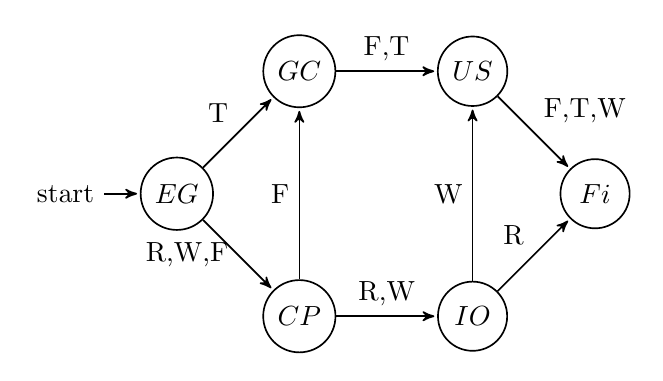
\begin{tikzpicture}[->,>=stealth',shorten >=1pt,auto,node distance=2.2cm,semithick]
%\tikzstyle{every state}=[fill=red,draw=none,text=white]

  \node[initial left,state] (A)              {$EG$};
  \node[state]         (B) [below right of=A] {$CP$};
  \node[state]         (D) [right of=B]       {$IO$};
  \node[state]         (C) [above right of=A] {$GC$};
  \node[state]         (E) [right of=C]       {$US$};
  \node[state]         (F) [below right of=E] {$Fi$};

  \path (A) edge        node [left] {R,W,F} (B)
            edge        node {T}     (C)
        (B) edge        node {F}     (C)
            edge        node {R,W}   (D)
        (C) edge        node {F,T}   (E)
        (D) edge        node {W}     (E)
            edge        node {R}     (F)
        (E) edge        node {F,T,W} (F);
\end{tikzpicture}
\caption{State transition diagram for read ($R$), write ($W$), fill ($F$), and
trim ($T$) CORFU operations. The states epoch guard ($EG$), check position ($CP$),
and update state ($US$) access metadata. The I/O performs a log entry read or
write, and garbage collection ($GC$) marks entries for reclamation.}
\label{fig:corfu-sm}
\end{figure}

The primary concern of an application developer when implementing an object
interface in Ceph is deciding how native interfaces are composed into a
compound operation. These types of decisions are commonly referred to as
physical design, and can affect performance and application flexibility.  For
instance, one valid design option is to store each log position in an object
with a name using a one-to-one mapping with the log entry position.  This
would simplify the design of the \emph{write} interface because a small amount
of metadata stored as a header in the object could describe the state of the
log entry.  However, as we will see in the next section this choice of a
physical design can result in poor performance compared to other designs.

\subsection{Physical Design}

As we have seen, Ceph provides a rich storage API and places few restrictions
on the structure of applications. So how should we go about implementing CORFU
on Ceph? Our strategy is straightforward: first we will define the entire
design space, and we will then winnow down this space using a set of targeted
benchmarks. The design space can be divided into three challenges:
selecting a strategy for log entry addressing, choosing a native I/O interface
for storing log entry content, and implementing efficient metadata management.

\begin{enumerate}
    \item {\bf Entry addressing.} We refer to the method by which a client
        locates a log entry in Ceph as entry addressing, and we consider two
        strategies. In a one-to-one (1:1) strategy each log entry is stored in
        a distinct object with a name derived from the associated log entry
        position. This is an attractive option because it is trivial for
        clients to locate a log entry given its position.  In contrast, an N:1
        strategy \emph{stripes} log entires across a smaller set of objects,
        but this adds complexity to both the client and the object interface which
        must multiplex a set of entries.

    \item {\bf Log entry storage.} Clients read and write binary data
        associated with each log entry, and these entries can be stored in the
        bytestream or in the key-value database associated with an object.
        Retrieval of log entry payloads should perform well for both large
        (e.g. database checkpoint) and small log entries.

    \item {\bf Metadata management.} The CORFU protocol defines the storage
        interface semantics, such as enforcing up-to-date epoch values and a
        write-once address space. The object interface constructed in Ceph must
        implement these semantics in software by storing metadata (e.g. the
        current epoch) and validating requests against this metadata (e.g. has
        the target position been written?). A key-value store is a natural
        location for this type of data, but metadata management adds overhead
        to each request and must be carefully designed.
\end{enumerate}

In the remainder of this section we will explore the full design space defined
by the cross product of these design challenges to arrive at a final design.

\paragraph*{Baseline Entry Storage Performance}
We begin the process of exploring the design space by exploiting the fact that
metadata management is a complexity and performance overhead that a full
implementation must incur beyond the costs of storing log entry data.
Therefore we first explore the design space by restricting the
space to log entry addressing and log entry storage.  These two dimensions are
represented by the first two columns of Table~\ref{tab:pd-map} which describes
the entire design space. In the I/O column \emph{KV} corresponds to the
key-value interface, and the bytestream interface is represented by \emph{AP}
for an append strategy, and \emph{EX} for a strategy that writes to an
explicit bytestream offset (both described shortly).

Figure~\ref{fig:vanilla_wr_jewel} shows the expected performance of 1K log
appends without metadata management overhead using each of the five strategies
defined in Table~\ref{tab:pd-map}. The first thing to notice in this figure is
that both one-to-one strategies have relatively poor performance. The large
period of reduced throughput for \emph{11wr} corresponds to the OSD splitting
file system directories in order to maintain a maximum directory size, and
will occur in \emph{11kv} although the threshold number of objects is not
reached in this example due to reduced overall throughput of the \emph{11kv} strategy.

The second lesson that we can learn from Figure~\ref{fig:vanilla_wr_jewel} is
that even when using an N:1 addressing strategy, the key-value interface
imposes a large overhead. This is unfortunate because the key-value interface
can provide a direct solution to addressing log entries within an object.
Instead, what we find is that an N:1 addressing strategy that stores log
entries in the bytestream using either object appends or writes to explicit
offsets outperform all other strategies by a factor of over 2x.

The apparent performance tie between the strategies of appending to an object
and writing to explicit offsets can be broken by considering the flexibility
offered by each approach. The third column \emph{entry size} in
Table~\ref{tab:pd-map} shows if a particular strategy supports storage of
entries with dynamic sizes, or if entries must be restricted to a fixed size.
Notably the strategy that stores log entries at explicit object offsets is
limited in this regard because each log entry is effectively pre-mapped into
the storage system. This leaves the clear winner: an N:1 strategy that appends
log entries to objects provides flexibility and the best write performance in
this particular configuration.  This result is corroborated by considering the
read performance for each strategy as well. Figure~\ref{fig:vanilla_rd_jewel}
shows the expected random read performance from a log containing 1K entries in
which an addressing strategy that stores log entries in the bytestream has the
best performance.

\begin{figure}[t]
  \centering
  \begin{subfigure}[b]{.47\linewidth}
      \centering
      \includegraphics[width=1.0\linewidth]{experiments/librados-sweep/jewel_ssd.png}
      \caption{1hr,1k,wr}
      \label{fig:vanilla_wr_jewel}
  \end{subfigure}\quad
  \begin{subfigure}[b]{.47\linewidth}
      \centering
      \includegraphics[width=1.0\linewidth]{experiments/basic-cls-rand-read/output.read.60min.1k.png}
      \caption{1hr,1k,rd}
      \label{fig:vanilla_rd_jewel}
  \end{subfigure}
  \caption{Ceph and OSD... gotta cram more stuff in here...}
\end{figure}

\begin{table}
\begin{tabular}{ | l | l | l | l | l |}
\hline
Map & I/O & Entry Size & Addressing & Metadata \\ \hline
\multirow{3}{*}{1:1} & KV  & Flex     & Ceph      & KV/BS \\ \cline{2-5}
                     & AP  & Flex     & Ceph/VFS  & KV/BS \\ \hline
\multirow{4}{*}{N:1} & KV  & Flex     & \multicolumn{2}{|c|}{KV/BS} \\ \cline{2-5}
                     & EX  & Fixed    & VFS       & KV/BS \\ \cline{2-5}
                     & AP  & Flex     & KV/BS     & KV/BS \\
\hline
\end{tabular}
\caption{The high-level design space of mapping CORFU log entry storage onto
the RADOS object storage system.}
\label{tab:pd-map}
\end{table}

\paragraph*{Metadata Management}

Adds in indexing and that sort of overheads.

\paragraph*{Hardware and Software}

Different hardware and different Ceph versions.

\section{Programming Model}

In this section we are going to be describing our way of creating interfaces.

\section{Other Interfaces}

Here we show the derivation of two other interfaces that are in production in
Ceph today to demonstrate the generality of our interface.

\section{Evaluation}

\section{Related Work}

\section{Conclusion}

%In this section we examine the design space for implementing the CORFU
%protocol in the RADOS storage system. Table \ref{t:init-ds} shows the entire
%design space. A description of each design parameter follows:
%
%{\bf Mapping strategy.} The method by which a log entry---identified by its
%logical position---is addressed within RADOS is referred to as the mapping
%strategy. A 1:1 strategy stores each log entry in a RADOS object with a
%distinct name (e.g. ``mylog.pos443''), and an N:1 strategy stripes the log
%positions across a set of objects (e.g.  round-robin). While we do consider
%both strategies in this paper, a 1:1 strategy is attractive because it allows
%a design in which clients can directly address log positions by constructing
%the correct object name.
%
%{\bf Storage interface.} entry data may be small or large. its primary
%storage location is important. kv, bs. we further sub-divide bs into
%write and append. each strategy is compatible with fixed size entries
%except for the write interface.
%
%{\bf Logical addressing.}

%\subsection{Storage Interface Selection}
%
%Figure \ref{f:librados-sweep} shows the single-node write-only I/O throughput
%for each of the points in the design space defined in Table \ref{t:init-ds}.
%The results reveal poor relative performance using both the key-value storage
%interface, as well as either of the 1:1 strategies---which incur overhead by
%creating a new object for each log entry. Both of the N:1 strategies using the
%bytestream I/O interface outperform all of the other approaches by over 2x
%throughput, but otherwise have nearly identical performance.
%
%To examine the read performance of the points in the design space we generated
%a dataset using each of the write workloads, and then issued random reads
%across the entire dataset. Figure \ref{f:librados-rand-read} shows the read
%throughput for each of the design strategies. The results show that an N:1
%mapping using bytestream interface performs best. Interestingly, the 1:1
%mapping strategy using the bytestream interface exhibits good read performance
%in comparison to writes using the same strategy.

%\begin{figure}[h]
%  \centering
%  \includegraphics[width=0.45\textwidth]{experiments/librados-sweep/output.soft.reset.2hr.png}
%  \caption{
%[\href{https://github.com/noahdesu/zlog-popper/tree/master/experiments/librados-sweep/visualize.ipynb}{source}]
%Throughput (IOPS) of 1K writes to a single OSD using the standard I/O
%interfaces in various configurations. The best performance is achieved using
%the byte stream interface and a N:1 mapping strategy.
%}
%\end{figure}
%
%\begin{figure}[h]
%  \centering
%  \includegraphics[width=0.45\textwidth]{experiments/basic-cls-rand-read/output.read.60min.png}
%  \caption{
%[\href{https://github.com/noahdesu/zlog-popper/tree/master/experiments/basic-cls-rand-read/visualize.ipynb}{source}]
%Throughput of 1K random reads to a single OSD using the standard I/O
%interfaces in various configurations. The best performance is achieved using
%the byte stream interface and a N:1 mapping strategy.
%}
%\end{figure}
%
%\begin{figure}[h]
%  \centering
%  \includegraphics[width=0.45\textwidth]{experiments/basic-cls-overhead/output.1024.soft.reset.png}
%  \caption{
%[\href{https://github.com/noahdesu/zlog-popper/tree/master/experiments/basic-cls-overhead/visualize.ipynb}{source}]
%}
%\end{figure}


%As a first approximation these results show that when optimizing for log
%append and random read throughput the design space should be refined by
%limiting solutions to architectures based on a N:1 mapping strategy using the
%bytestream I/O interface. But what these microbenchmarks explicitly omit are
%the overheads associated with metadata management such as enforcing write-once
%semantics or using an index to map a log position to a physical offset within
%an object. In the next section we

\bibliography{paper}
\bibliographystyle{plain}

\end{document}
